%! Author = breandan
%! Date = 2/22/24

% Preamble
\documentclass[11pt]{article}

% Packages
\usepackage{amsmath}

\usepackage{tikz}
\usepackage{amssymb}
\usetikzlibrary{shapes.geometric, arrows}

\tikzstyle{startstop} = [rectangle, rounded corners,
minimum width=3cm,
minimum height=1cm,
text centered,
draw=black,
fill=red!30]

\tikzstyle{io} = [trapezium,
trapezium stretches=true, % A later addition
trapezium left angle=70,
trapezium right angle=110,
minimum width=3cm,
minimum height=1cm, text centered,
draw=black, fill=blue!30]

\tikzstyle{process} = [rectangle,
minimum width=3.5cm,
minimum height=1cm,
text centered,
text width=3.5cm,
draw=black,
fill=orange!30]

\tikzstyle{decision} = [diamond,
minimum width=3cm,
minimum height=1cm,
text centered,
draw=black,
fill=green!30]
\tikzstyle{arrow} = [thick,->,>=stealth]
\begin{document}

% Document
\begin{document}

\section{Method}

The syntax of most programming languages is context-free. Our proposed method is simple. We construct a context-free grammar representing the intersection between the langauge syntax and an automaton recognizing the Levenshtein edit ball up to a fixed distance. Since CFLs are closed under intersection with regular languages, this is admissible. Three outcomes are possible:

\begin{enumerate}
  \item $\mathcal{G}_\cap$ is empty, in which case there is no repair within the given radius. In this case, we simply increase the radius and try again.
  \item $\mathcal{G}_\cap$ is small, in which case we simply enumerate all possible repairs. This is the case for ~80\% of the Python dataset.
  \item $\mathcal{G}_\cap$ is too large to exhaustively sample, in which case we use a PCFG to sample $\mathcal{L}(\mathcal{G})$ without replacement, then reject duplicates. This is the case for ~20\% of the Python dataset.
\end{enumerate}

After sampling, we use an n-gram model to rank the samples, then return the top-k results by likelihood. We depict the flowchart below:

\begin{figure}[h!]
  \begin{center}
\resizebox{0.6\textwidth}{!}{
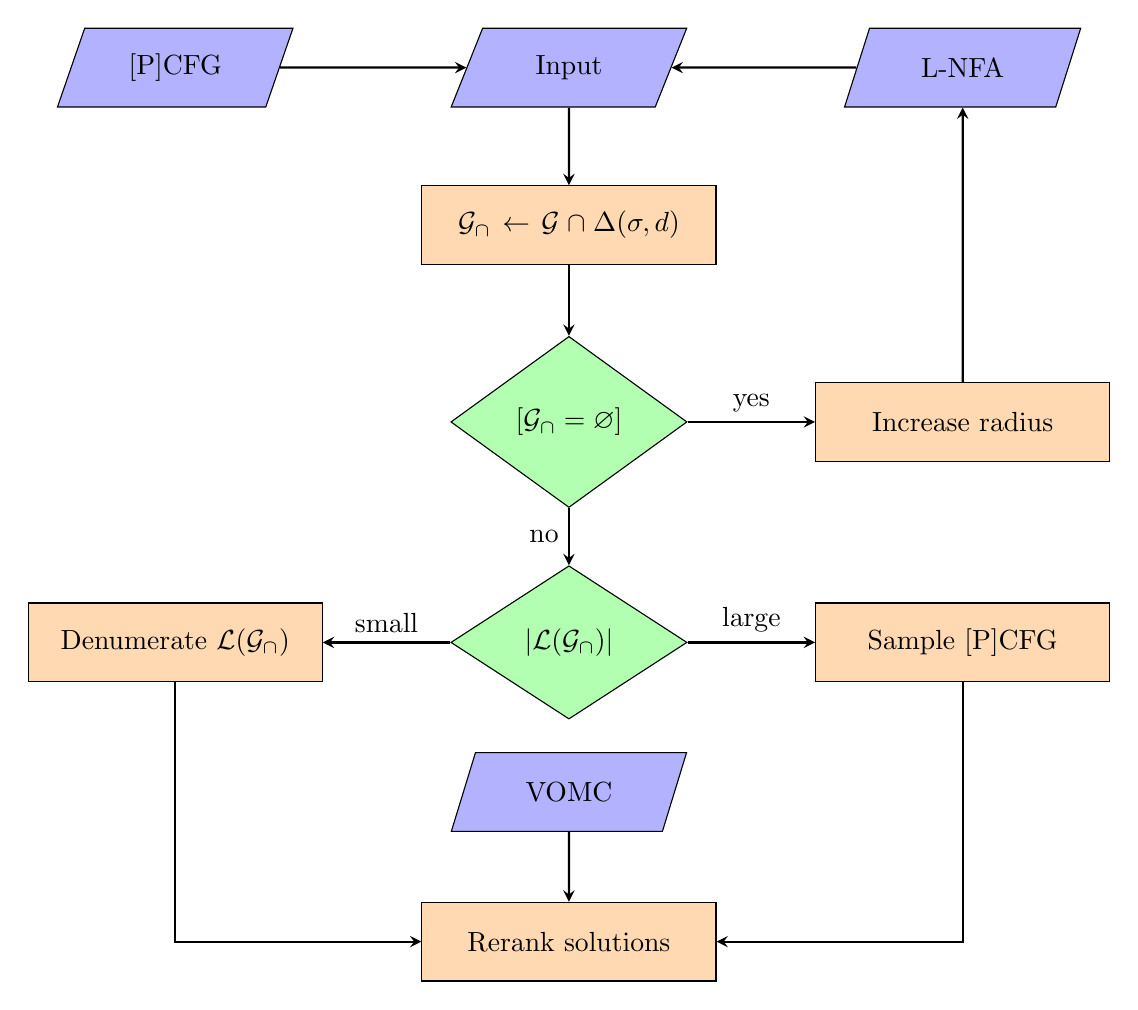
\begin{tikzpicture}[node distance=2cm]

%  \node (start) [startstop] {Start};
  \node (in1) [io] {Input};
  \node (rin1) [io, right of=in1, xshift=3cm] {L-NFA};
  \node (lin1) [io, left of=in1, xshift=-3cm] {[P]CFG};

  \node (pro1) [process, below of=in1] {$\mathcal{G}_\cap \leftarrow \mathcal{G}\cap\Delta(\err\sigma, d)$};

  \node (dec1) [decision, below of=pro1, yshift=-0.5cm] {$[\mathcal{G}_{\cap} = \varnothing]$};

  \node (pro2b) [process, right of=dec1, xshift=3cm] {Increase radius};

  \node (dec2) [decision, below of=dec1, yshift=-0.8cm] {$|\mathcal{L}(\mathcal{G}_\cap)|$};

  \node (samp1) [process, left of=dec2, xshift=-3cm] {Denumerate $\mathcal{L}(\mathcal{G}_\cap)$};
  \node (samp2) [process, right of=dec2, xshift=3cm] {Sample [P]CFG};

  \node (uin1) [io, below of=dec2, yshift=0.1cm] {VOMC};
  \node (rank1) [process, below of=uin1, yshift=0.1cm] {Rerank solutions};

%  \node (out1) [io, below of=pro2a] {Output};
%  \node (stop) [startstop, below of=out1] {Stop};

%  \draw [arrow] (start) -- (in1);

  \draw [arrow] (rin1) -- (in1);
  \draw [arrow] (lin1) -- (in1);

  \draw [arrow] (in1) -- (pro1);
  \draw [arrow] (pro1) -- (dec1);
  \draw [arrow] (dec1) -- node[anchor=south] {yes} (pro2b);
  \draw [arrow] (dec1) -- node[anchor=east] {no} (dec2);
  \draw [arrow] (pro2b) -- (rin1);
  \draw [arrow] (dec2) -- node[anchor=south] {small} (samp1);
  \draw [arrow] (dec2) -- node[anchor=south] {large} (samp2);

  \draw [arrow] (uin1) -- (rank1);
  \draw [arrow] (samp1) |- (rank1);
  \draw [arrow] (samp2) |- (rank1);
%  \draw [arrow] (pro2a) -- (out1);
%  \draw [arrow] (out1) -- (stop);

\end{tikzpicture}
}
\end{center}
\caption{Flowchart of our proposed method.}\label{fig:flowchart}
\end{figure}

\end{document}